\chapter{Experimentos y evaluación}
\label{cap:experimentos}

\section{Implementación del sistema}
%Acá hay que hablar de todo lo que implementaste a grandes rasgos (detalles Anexo), modelo, manejo de réplicas, etc. Redactar de nuevo

Para la implementanción del sistema propuesto, se utilizó como base el motor de procesamiento de \textit{stream} S4 \citep{s4}, cuyo modelo fue explicado en la sección \ref{sec:SPS}. El funcionamiento del sistema de distribución de carga propuesto se desarrolló en Java, donde se modificó en el código fuente de S4, para incluir las funciones de este producto, de tal manera que fuera automático y transparente para el usuario del SPS.

El sistema diseñado fue añadido al proyecto S4, siendo una paquete denominado \textit{monitor} que contenía las clases \textit{S4Monitor}, \textit{MarkovChain}, \textit{MonitorMetrics}, \textit{StatusPE} y \textit{TopologyApp}. La primer clase correspondía a las funcionalidades del sistema de monitoreo, ya sea la recepción de los datos del sistema, ejecución del algoritmo reactivo o predictivo y administración de las réplicas de cada operador. La segunda clase hacía alusión al modelo de cadena de Markov implementando por el algoritmo predictivo, donde posee tanto la conformación de la matriz de transición como el cálculo de la distribución estacionaria. La tercera clase se utilizó para recolectar las estadísticas de cada operador, y poder analizar los experimentos. Finalmente, la cuarta y quinta clase fueron utilizadas para la implementación del sistema de monitoreo, siendo la primera el estado de cada PE y el segundo la topología que poseía el grafo creado por el usuario, los cuales pueden verse con más detalle en el Anexo \ref{apendice:clases}.

Por otra parte, para el análisis de cada uno de los PEs, se añadió los atributos de cantidad de eventos entrantes y salientes cada un segundo y cinco segundos. Esto fue utilizado posteriormente para las estadísticas deseadas para el algoritmo reactivo y predictivo. La tasa de llegada es considerada desde el momento que se recibe el evento desde el PE emisor, y la tasa de servicio es considera desde el momento que se termina de realizar la ejecución de la tarea en el PE.

Por lo tanto, para el funcionamiento del sistema de distribución de carga se procedió a ejecutar dos tareas en la aplicación de S4: una tarea que guarde las muestras para el historial del operador y otra que envíe las estadísticas del operador, las cuales poseían un intervalo de ejecución de 1 y 5 segundos respectivamente. La primera tarea analiza cada uno de los PEs, tomando en consideración las estadísticas de eventos entrantes y salientes, los cuales darán origen a la tasa de llegada ($\lambda$) y servicio ($\mu$), para que posteriormente se calcule la tasa de rendimiento en la ventana de tiempo analizada, guardando así la muestra en el historial. La segunda tarea obtiene las estadísticas de cada uno de los PEs, ya sea la tasa de llegada ($\lambda$) y servicio ($\mu$), dado los eventos entrantes y saliente, cantidad de eventos totales e historial del PE, los cuales son enviados al monitoreo de carga, para posteriormente ejecutar el algoritmo que corresponda según la ventana de tiempo.

Debido al funcionamiento de los SPS, existe una fuente de datos, por lo tanto, para la correcta sincronización de las estadísticas, se procedió a realizar una espera por parte del monitor hasta que la fuente de datos esté lista para enviar los datos. Esta implementanción se puede ver en el Anexo \ref{apendice:codigoFuenteS4}, conjunto con las dos tareas que debe ejecutar después que la fuente de datos avisa de su inicialización.

En el caso del envío de las estadísticas, después de ser enviadas, se consulta el estado de cada uno de los operadores, y en caso de ser necesario, se realiza las modificaciones necesarias en el sistema, ya sea de crear o eliminar réplicas de un operador. En el caso de crear réplicas, lo que se realiza es consultar la cantidad de réplicas que dijo que debían existir por parte del administrador de réplicas, y en caso de poseer un número de réplicas mayor que el existente por el PE, se procede a crear la cantidad de réplicas faltantes. Por otra parte, en caso de que el número sea menor, procede a terminar la ejecución del PE y posteriormente elimina la cantidad de réplicas sobrantes. Los códigos de crear o eliminar replicas se encuentra adjuntos en el Anexo \ref{apendice:codigoFuenteS4}.

Dado que en el diseño se propuso un mecanismo de balance de carga basado en la técnica de replicación, fue necesario modificar S4, de manera de poder manejar las réplicas para los operadores. Se implementó el SPS de tal manera de poder manejar un algoritmo que escogiera la réplica que tuviera menor tamaño en la cola de espera al momento de enviar un dato, y así siempre escoger al operador con menor carga, y en caso que posean el mismo tamaño, utilizar la primera réplica disponible.

En la Figura \ref{fig:distCarga} se explica gráficamente la distribución de la carga. En la parte (a) el operador A envía un evento al operador B, el cual posee tres réplicas, cuyas menores colas están en la réplica 2 y 3, como son iguales las colas de estas réplicas, se escoge la primera réplica disponible, es decir, la réplica 2. Posteriormente, como la réplica 2 aumento su cola, la réplica 3 es la que posee menor cantidad de cola, como se demuestra en la parte (b), por lo tanto, es la réplica candidata a recibir el dato enviado. Y finalmente, en la parte (c) todas las réplicas posee el mismo tamaño de la cola, por lo tanto, se procede a enviar a la primera réplica.

\begin{figure}[!ht]
	\centering
		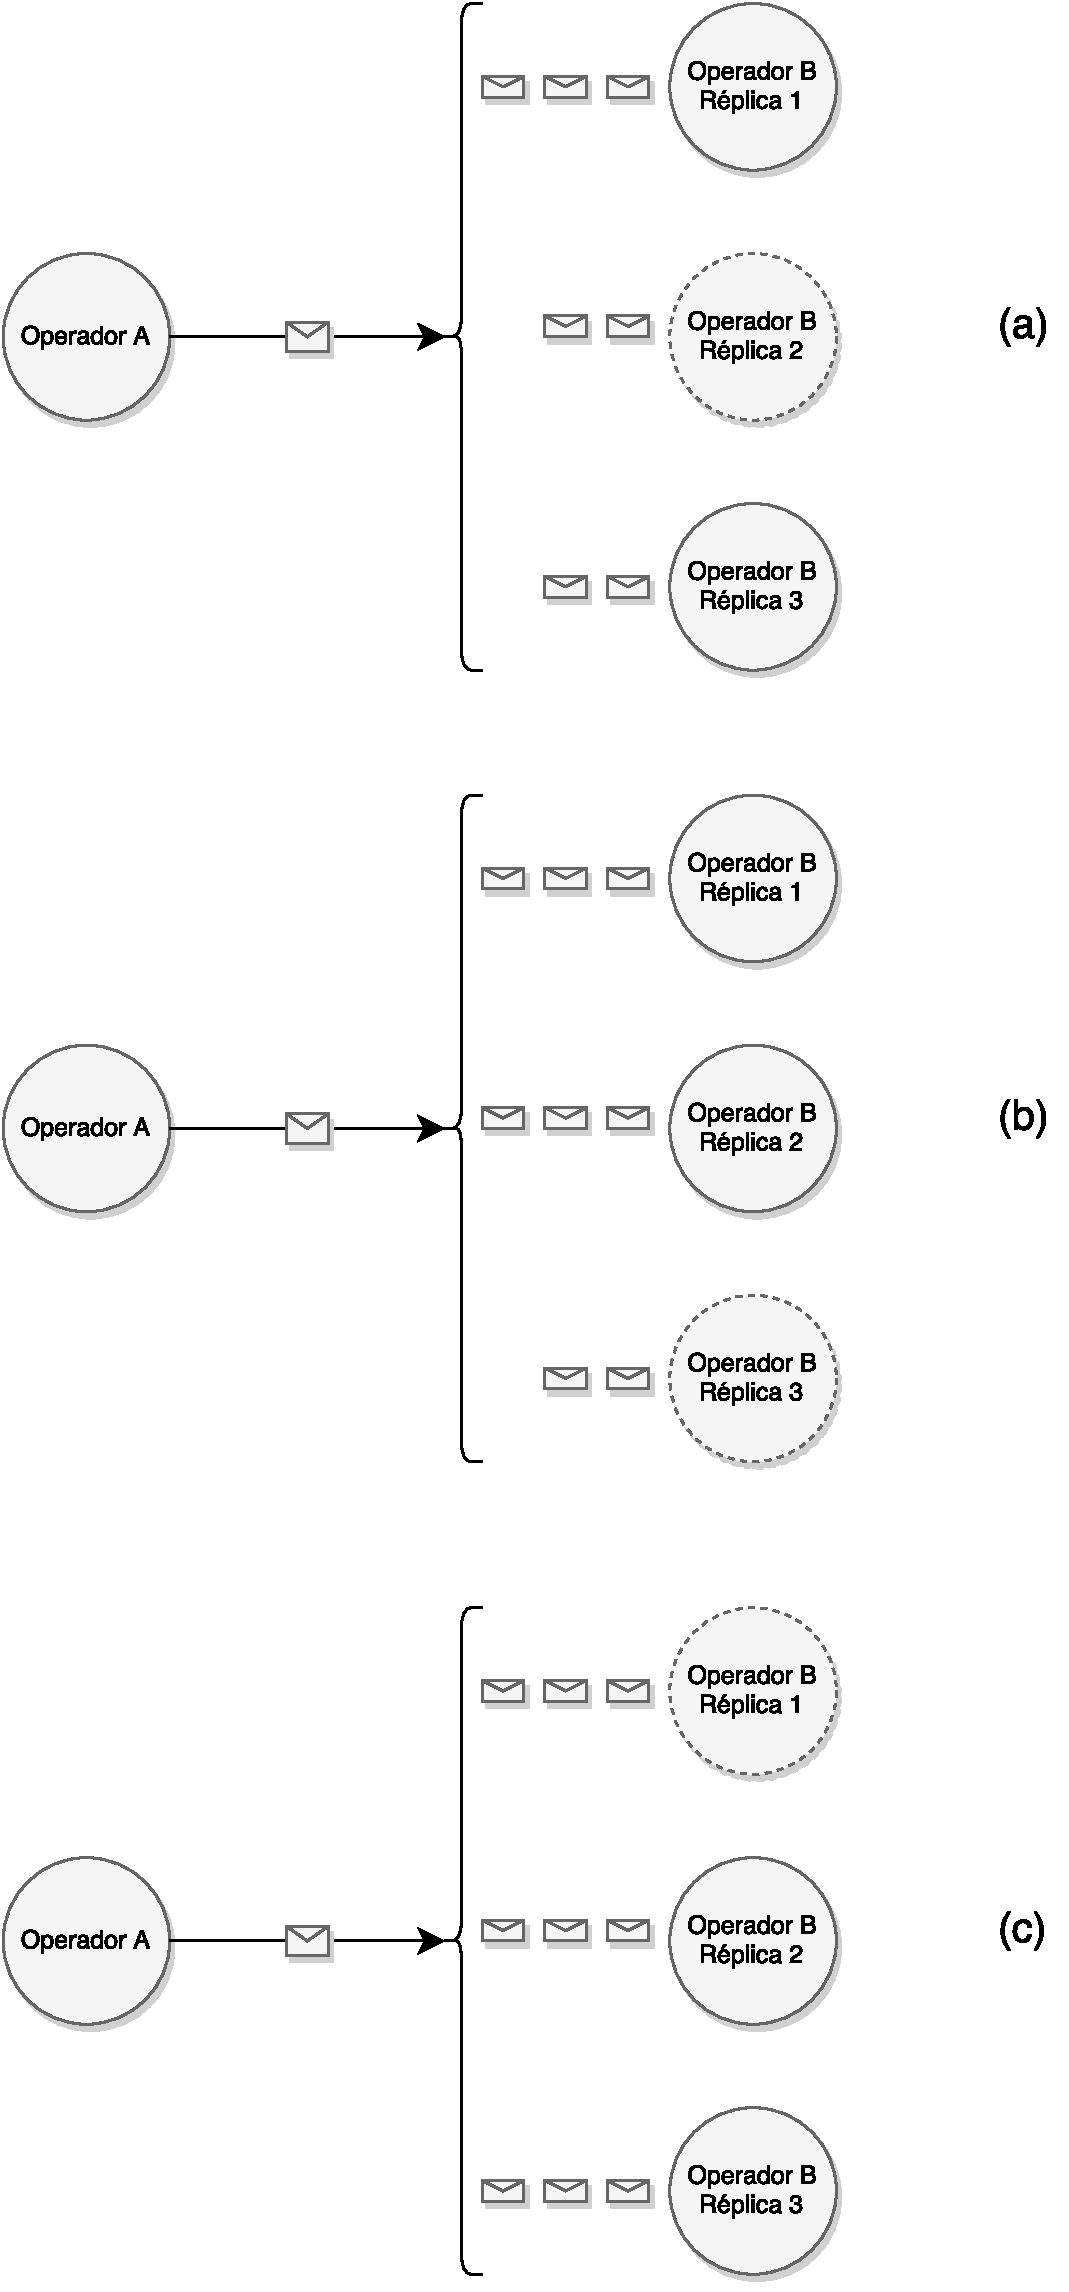
\includegraphics[scale=0.55]{images/DistribucionCarga.pdf}
	\caption{Distribución de la carga entre las réplicas.}
	\label{fig:distCarga}
\end{figure}

En el Algoritmo \ref{alg:distCarga} está descrito la distribución de carga planteada anteriormente, la cual fue implementada en S4 para realizar los experimentos según lo diseñado en el planteamiento de los algoritmos.

\begin{algorithm}[!ht]
	\caption{Distribución de carga entre las réplicas de un operador.}
	\label{alg:distCarga}
	\begin{algorithmic}[1]
	\REQUIRE Evento $\epsilon$ y operador $\phi$.
	\ENSURE Envío del evento a la réplica disponible del operador $\phi$.
	\STATE $\theta \leftarrow minTamanoCola(\phi)$ \COMMENT Se escoge la réplica que posea menor cola
	\STATE $envioEvento(\epsilon,\theta$)
	\end{algorithmic}
\end{algorithm}

\section{Diseño de los experimentos}
Para los experimentos se diseñaron tres aplicaciones, una que realiza operaciones con estado, otra que no, y otra que es sintética. En el caso que la aplicación posea estado, significa que el operador guarda variables con el transcurso del tiempo, las cuales van a ser entregadas cada cierto tiempo o al finalizar la ejecución del sistema. Un ejemplo de esto, es un sistema que cuenta las palabras de un texto y que envié la cantidad de palabras contadas cada cierta ventana de tiempo. Por otra parte, la aplicación sintética se refiere a un sistema cuyos operadores sólo generan tiempo de demora artificial, en el caso de este experimento, se dejo durmiendo la hebra asignada al operador un período determinado de tiempo.

Para la generación del \textit{stream} de la fuenta de datos, se utilizaron datos de muestra utilizados fueron \textit{tweets} recolectados entre los días 27 y 28 de Febrero y 1 y 2 de Marzo de 2010, tanto en inglés, portugués y español, cuya información correspondía a la interacción entre los usuarios debido al terremoto ocurrido el 27 de Febrero en el territorio Chile.

\subsection{Análisis de \textit{tweets} en escenarios de desastres naturales}
La primera aplicación fue orientada a un caso de desastres naturales, donde se generó un grafo que pudiera realizar un filtrado de palabras y análisis de los datos. Ninguno de los operadores posee estado, por lo tanto son independientes.

La aplicación consta del flujo de datos, cuyos datos serán la muestra de \textit{tweets} de prueba, y cuatro operadores, los cual son denominados \textit{Stopword}, \textit{Language}, \textit{Counter} y \textit{MongoDB}.

\paragraph{Stopword}: está encargado de analizar el \textit{tweet} y remover las palabras no relevantes para el análisis de éste, basado en una bolsa de palabras, cuyas palabras se llaman \textit{stopwords}. De esta manera, se puede analizar el texto usando las palabras más representativas de éste y así entregar información más precisa.

\paragraph{Language}: está encargado de analizar el lenguaje existente en el \textit{tweet}, para esto se utilizó una librería \textit{Apache Tika} \citep{mattmann2011tika}. Con ésta se puede realizar un filtro del idioma de los tweets, de tal manera que en caso de ser requerido, sólo continúen los de un idioma en específico, en nuestro caso el español.

\paragraph{Counter}: está encargado de contar e indicar la cantidad de palabras que existen en el \textit{tweet} según una bolsa de palabras proporcionada por el programador. Para esta prueba se utilizó una bolsa de 26.000 palabras en español. Con esto se podría realizar un análisis de los \textit{tweets} que poseían mayor cantidad de palabras claves asociados a una temática o evento en particular.

\paragraph{MongoDB}: está encargado de guardar en la base de datos el evento según los atributos que éste posea, ya sea por el \textit{tweet} original, sin \textit{stopword}, idioma y cantidad de palabras claves existentes en él. Para esto, se utilizó el motor de base de datos no relacional \textit{MongoDB} \citep{chodorow2013mongodb}.

En la Figura \ref{fig:primeraAplicacion} se muestra un ejemplo de la aplicación con sus distintos operadores y relaciones. Las flechas muestran la dirección del flujo de datos emitido por la fuente y los operadores.

\begin{figure}[!hb]
	\centering
		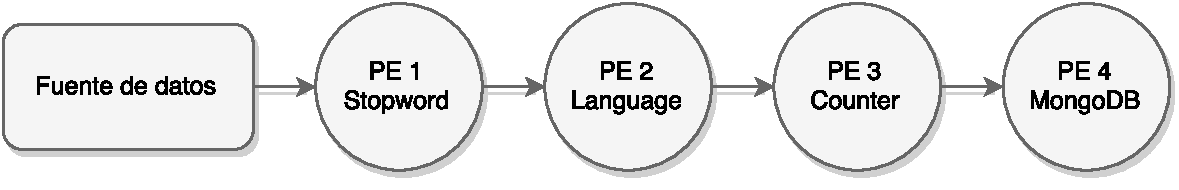
\includegraphics[scale=0.75]{images/App1.pdf}
	\caption{Primera aplicación de prueba.}
	\label{fig:primeraAplicacion}
\end{figure}

\subsection{Contador de palabras en muestras de textos}
La segunda aplicación consiste en un contador de palabras, el cual cuenta la cantidad de veces que se repite una palabra en un conjunto de datos según una bolsa de palabras establecida por el usuario. Esta aplicación se considera con estado, debido que debe existir un contador en el operador, de tal manera de contar la cantidad de veces que se repite cierta palabra de la bolsa de palabras en los datos entrantes. Con esta aplicación es posible analizar posteriormente las palabras más frecuentes emitidas por los usuarios de la red social según un listado de palabras claves.

La aplicación consta del flujo de datos, cuyos datos serán la muestra de \textit{tweets} de prueba, y tres operadores, denominados \textit{Split}, \textit{Counter} y \textit{Merge}.

\paragraph{Split} Está encargado de dividir el \textit{tweet}, y enviar un arreglo con las palabras que poseía este texto al operador \textit{Counter}.

\paragraph{Counter} Está encargado de guardar las estadísticas de los contadores de cada palabra, es decir, en el momento que reciba un evento, este analiza las palabras que posee y aumenta el contar de la palabra en el operador. Las estadísticas son enviadas cada 10 segundos al operador Merge, de tal manera de no enviar flujo constante al siguiente operador y generar mayor cantidad de carga.

\paragraph{Merge} Está encargado de unir las distintas estadísticas enviadas por las distintas réplicas del operador Counter.

En la Figura \ref{fig:primeraAplicacion} se muestra un ejemplo de la segunda aplicación con sus distintos operadores y sus relaciones, de igual manera que en el caso anterior, las flechas reflejan el flujo de datos. Cabe destacar que el único operador que puede replicarse es el \textit{Counter}, debido que el operador \textit{Split} y \textit{Merge} son operadores que soportan la replicación del operador \textit{Counter}, como se explicó en las técnicas de balance de carga en la subsección \ref{sec:fisionBC}.

\begin{figure}[!hb]
	\centering
		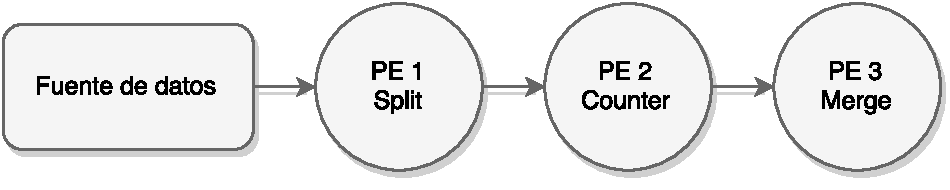
\includegraphics[scale=0.75]{images/App2.pdf}
	\caption{Segunda aplicación de prueba.}
	\label{fig:segundaAplicacion}
\end{figure}

\subsection{Aplicación sintética}
La tercera aplicación consta de tres operadores, los cuales 

\section{Evaluación}

Para la ejecución de los experimentos, se utilizó un servidor con sistema operativo Ubuntu 14.04.2 LTS, cuyo procesador es un Intel\textregistered Xeon\textregistered CPU E5-2650 v2 de 2.60GHz y con 32 GB de RAM. Cabe recalcar, que el lenguaje de programación fue Java, debido a la integración del sistema propuesto en el SPS utilizado, el cual fue S4.

